\hypertarget{polygon-triangulation}{%
\section{Polygon Triangulation}\label{polygon-triangulation}}

\hypertarget{introduction}{%
\subsection{Introduction}\label{introduction}}

The decomposition of a polygon into triangles whose union again results
in the original polygon is called polygon triangulation. In the method,
no new Vertices are added. Only the diagonals of the polygon results in
the triangulation. There need not be a unique triangulation for a given
polygon.

There are various methods which can be used to perform polygon
triangulation. In our implementation, we
\protect\hyperlink{algorithm-approach}{discuss} two types of
triangulation which are: 1) Ear Clipping Triangulation. 2) Plane sweep
monotone division combined with Monotone triangulation.

\hypertarget{how-to-run}{%
\subsection{How to Run}\label{how-to-run}}

The src folder contains the source code for the convex hull program.
\texttt{g++} from the GNU compiler suite is required to compile the
program to a executable.

Steps to Compile:

\begin{enumerate}
\def\labelenumi{\arabic{enumi})}
\tightlist
\item
  \texttt{cd} into the src directory
\item
  Run \texttt{g++\ main.cpp} which generates an executable called
  \texttt{a.out} in the same directory
\item
  Run the executable using \texttt{./a.out} (on linux)

  \begin{enumerate}
  \def\labelenumii{\arabic{enumii})}
  \tightlist
  \item
    The executable takes a dataset from command line argument. For
    example, to use an existing dataset, run
    \texttt{./a.out\ ../datasets/complex.txt}
  \item
    If no command-line argument is given, it takes input from the shell
    directly (stdin)
  \end{enumerate}
\end{enumerate}

\hypertarget{input}{%
\subsection{Input}\label{input}}

The required file format for the algorithm to work correctly is:

\begin{itemize}
\tightlist
\item
  The input \textbf{must} be a clockwise ordering of Poins present on
  the polygon.
\item
  First line must contain the no of Points to be taken as input by the
  program.
\item
  Each of next line must contain 2 integers, space seperated denoting
  the (x, y) coordinates of each point.
\item
  Each coordinate must be of integer type in the range -10\^{}8 to
  10\^{}8.
\item
  No of coordinates must be less than 1 Billion.
\end{itemize}

\hypertarget{output}{%
\subsection{Output}\label{output}}

Each line of output contains three coordinates of points present on each
triangulation.\\
The last two lines of output show the time taken to take input in
microseconds and the time taken by the algorithm to compute
Triangulation (also in microseconds).

This is the output of one of the datasets
\href{./datasets/long.txt}{long.txt}

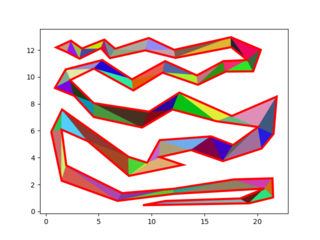
\includegraphics[width=8cm,height=8cm]{img/TRIsnake.png}\\

\hypertarget{documentation-and-report}{%
\subsection{Documentation and Report}\label{documentation-and-report}}

Documentation of this algorithm, functions and classes can be found in
the \texttt{docs} folder in the current directory. Open the
\href{../Triangulation/docs/html/index.html}{index.html} file from the
docs directory with your preferred browser to go through the
documentation

\hypertarget{performance-analysis}{%
\subsection{Performance Analysis}\label{performance-analysis}}

Analysis is performed with a system running (does not include printing
time):

\begin{itemize}
\tightlist
\item
  OS: Arch Linux (64Bit) running Linux Kernel version 5.7.2
\item
  Processor: Intel Core i7 7700HQ
\item
  RAM: 8GB
\item
  Compiler: GNU G++ (GCC) 10.1.0
\end{itemize}

\textbf{The following observations are recorded:}

Time taken to triangulate basic shapes:

\begin{longtable}[]{@{}lcccc@{}}
\toprule
\begin{minipage}[b]{0.07\columnwidth}\raggedright
Filename\strut
\end{minipage} & \begin{minipage}[b]{0.12\columnwidth}\centering
Input Vertices\strut
\end{minipage} & \begin{minipage}[b]{0.15\columnwidth}\centering
Computed Triangles\strut
\end{minipage} & \begin{minipage}[b]{0.25\columnwidth}\centering
Line Sweep Triangulation Runtime\strut
\end{minipage} & \begin{minipage}[b]{0.27\columnwidth}\centering
Ear Clipping Triangulation Runtime\strut
\end{minipage}\tabularnewline
\midrule
\endhead
\begin{minipage}[t]{0.07\columnwidth}\raggedright
triangle.txt\strut
\end{minipage} & \begin{minipage}[t]{0.12\columnwidth}\centering
3\strut
\end{minipage} & \begin{minipage}[t]{0.15\columnwidth}\centering
1\strut
\end{minipage} & \begin{minipage}[t]{0.25\columnwidth}\centering
30 microsec\strut
\end{minipage} & \begin{minipage}[t]{0.27\columnwidth}\centering
16 microsec\strut
\end{minipage}\tabularnewline
\begin{minipage}[t]{0.07\columnwidth}\raggedright
downConvex.txt\strut
\end{minipage} & \begin{minipage}[t]{0.12\columnwidth}\centering
6\strut
\end{minipage} & \begin{minipage}[t]{0.15\columnwidth}\centering
4\strut
\end{minipage} & \begin{minipage}[t]{0.25\columnwidth}\centering
43 microsec\strut
\end{minipage} & \begin{minipage}[t]{0.27\columnwidth}\centering
23 microsec\strut
\end{minipage}\tabularnewline
\begin{minipage}[t]{0.07\columnwidth}\raggedright
test.txt\strut
\end{minipage} & \begin{minipage}[t]{0.12\columnwidth}\centering
6\strut
\end{minipage} & \begin{minipage}[t]{0.15\columnwidth}\centering
4\strut
\end{minipage} & \begin{minipage}[t]{0.25\columnwidth}\centering
35 microsec\strut
\end{minipage} & \begin{minipage}[t]{0.27\columnwidth}\centering
24 microsec\strut
\end{minipage}\tabularnewline
\begin{minipage}[t]{0.07\columnwidth}\raggedright
square.txt\strut
\end{minipage} & \begin{minipage}[t]{0.12\columnwidth}\centering
4\strut
\end{minipage} & \begin{minipage}[t]{0.15\columnwidth}\centering
2\strut
\end{minipage} & \begin{minipage}[t]{0.25\columnwidth}\centering
36 microsec\strut
\end{minipage} & \begin{minipage}[t]{0.27\columnwidth}\centering
18 microsec\strut
\end{minipage}\tabularnewline
\begin{minipage}[t]{0.07\columnwidth}\raggedright
hexagon.txt\strut
\end{minipage} & \begin{minipage}[t]{0.12\columnwidth}\centering
6\strut
\end{minipage} & \begin{minipage}[t]{0.15\columnwidth}\centering
4\strut
\end{minipage} & \begin{minipage}[t]{0.25\columnwidth}\centering
38 microsec\strut
\end{minipage} & \begin{minipage}[t]{0.27\columnwidth}\centering
16 microsec\strut
\end{minipage}\tabularnewline
\begin{minipage}[t]{0.07\columnwidth}\raggedright
monotone.txt\strut
\end{minipage} & \begin{minipage}[t]{0.12\columnwidth}\centering
15\strut
\end{minipage} & \begin{minipage}[t]{0.15\columnwidth}\centering
13\strut
\end{minipage} & \begin{minipage}[t]{0.25\columnwidth}\centering
109 microsec\strut
\end{minipage} & \begin{minipage}[t]{0.27\columnwidth}\centering
75 microsec\strut
\end{minipage}\tabularnewline
\begin{minipage}[t]{0.07\columnwidth}\raggedright
uniMonotone.txt\strut
\end{minipage} & \begin{minipage}[t]{0.12\columnwidth}\centering
8\strut
\end{minipage} & \begin{minipage}[t]{0.15\columnwidth}\centering
6\strut
\end{minipage} & \begin{minipage}[t]{0.25\columnwidth}\centering
115 microsec\strut
\end{minipage} & \begin{minipage}[t]{0.27\columnwidth}\centering
42 microsec\strut
\end{minipage}\tabularnewline
\begin{minipage}[t]{0.07\columnwidth}\raggedright
complex.txt\strut
\end{minipage} & \begin{minipage}[t]{0.12\columnwidth}\centering
17\strut
\end{minipage} & \begin{minipage}[t]{0.15\columnwidth}\centering
15\strut
\end{minipage} & \begin{minipage}[t]{0.25\columnwidth}\centering
188 microsec\strut
\end{minipage} & \begin{minipage}[t]{0.27\columnwidth}\centering
17 microsec\strut
\end{minipage}\tabularnewline
\begin{minipage}[t]{0.07\columnwidth}\raggedright
strange.txt\strut
\end{minipage} & \begin{minipage}[t]{0.12\columnwidth}\centering
16\strut
\end{minipage} & \begin{minipage}[t]{0.15\columnwidth}\centering
14\strut
\end{minipage} & \begin{minipage}[t]{0.25\columnwidth}\centering
148 microsec\strut
\end{minipage} & \begin{minipage}[t]{0.27\columnwidth}\centering
122 microsec\strut
\end{minipage}\tabularnewline
\begin{minipage}[t]{0.07\columnwidth}\raggedright
star.txt\strut
\end{minipage} & \begin{minipage}[t]{0.12\columnwidth}\centering
10\strut
\end{minipage} & \begin{minipage}[t]{0.15\columnwidth}\centering
8\strut
\end{minipage} & \begin{minipage}[t]{0.25\columnwidth}\centering
159 microsec\strut
\end{minipage} & \begin{minipage}[t]{0.27\columnwidth}\centering
101 microsec\strut
\end{minipage}\tabularnewline
\begin{minipage}[t]{0.07\columnwidth}\raggedright
spiral.txt\strut
\end{minipage} & \begin{minipage}[t]{0.12\columnwidth}\centering
32\strut
\end{minipage} & \begin{minipage}[t]{0.15\columnwidth}\centering
30\strut
\end{minipage} & \begin{minipage}[t]{0.25\columnwidth}\centering
278 microsec\strut
\end{minipage} & \begin{minipage}[t]{0.27\columnwidth}\centering
214 microsec\strut
\end{minipage}\tabularnewline
\begin{minipage}[t]{0.07\columnwidth}\raggedright
tank.txt\strut
\end{minipage} & \begin{minipage}[t]{0.12\columnwidth}\centering
55\strut
\end{minipage} & \begin{minipage}[t]{0.15\columnwidth}\centering
53\strut
\end{minipage} & \begin{minipage}[t]{0.25\columnwidth}\centering
429 microsec\strut
\end{minipage} & \begin{minipage}[t]{0.27\columnwidth}\centering
452 microsec\strut
\end{minipage}\tabularnewline
\begin{minipage}[t]{0.07\columnwidth}\raggedright
long.txt\strut
\end{minipage} & \begin{minipage}[t]{0.12\columnwidth}\centering
72\strut
\end{minipage} & \begin{minipage}[t]{0.15\columnwidth}\centering
70\strut
\end{minipage} & \begin{minipage}[t]{0.25\columnwidth}\centering
593 microsec\strut
\end{minipage} & \begin{minipage}[t]{0.27\columnwidth}\centering
1668 microsec\strut
\end{minipage}\tabularnewline
\bottomrule
\end{longtable}

\hypertarget{algorithm-approach}{%
\subsection{Algorithm Approach}\label{algorithm-approach}}

\hypertarget{ear-clipping}{%
\subsubsection{Ear Clipping}\label{ear-clipping}}

According to the two ears theorem, any simple polygon with minimum of 4
vertices without holes has atleast two ``ears''. An Ear is defined at
the vertex where internal angle is less than PI and the line joining the
adjacent vertices is a diagonal of the polygon.

The algorithm works by removing away these ``ears'' (which are
triangles) until the complete polygon is triangulated. This algorithm is
easy to implement, but slower than some other algorithms, and it only
works on polygons without holes. The runtime complexity of this
algorithm is O(n\textsuperscript{2})

\hypertarget{plane-sweep-monotone-triangulation}{%
\subsubsection{Plane Sweep Monotone
Triangulation}\label{plane-sweep-monotone-triangulation}}

A monotone polygon can be easily triangulated in O(n) complexity. A
simple polygon is said to be monotone w.r.t a line L only if any line
perpendicular to L passes through the polygon at most twice. Any
monotone polygon can be divided into two monotone chains. A polygon that
is monotone w.r.t the x-axis is called x-monotone. Given x-monotone
polygon, the greedy algorithm begins by walking on one chain of the
polygon from top to bottom while adding diagonals (forming triangles)
whenever it is possible.

If a polygon is not monotone, it can be partitioned into monotone sub
polygons in O(n log n) time using line/plane sweep method. Generally,
this algorithm can triangulate a planar subdivision with in O(n log n)
time using O(n) space.

\hypertarget{results}{%
\subsection{Results}\label{results}}

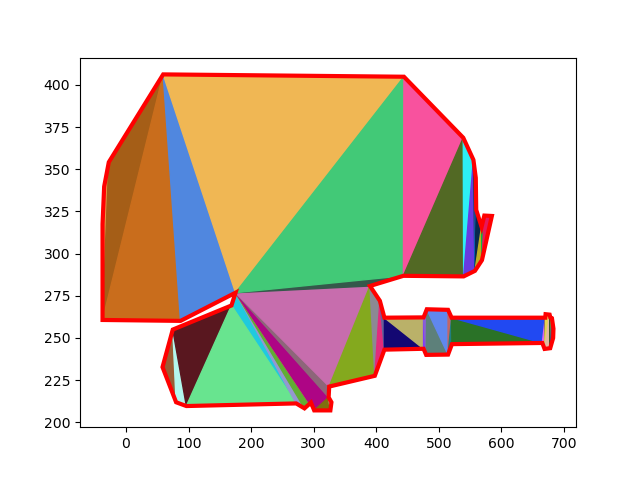
\includegraphics[width=8cm,height=8cm]{img/TRItank.png}\\

In the above image, the red boundary represents the input given to the
algorithm and the random colored triangle represent the output given by
the program.

It can be observed from the examples that increase in number of vertices
affects the runtime of ear clipping triangulation more than the plane
sweep monotone triangulation. From the results of the above datasets, we
can see that for just an increase of vertices from 50 to 70 causes the
ear clipping algorithm to triple its triangulation time.

\hypertarget{conclusion}{%
\subsection{Conclusion}\label{conclusion}}

From the above comparisions, we can see that ear clipping algorithm,
even after being a simple algorithm, due it is asymptotic complexity
being O(n\textsuperscript{2}), it surely is not recomended for
applications where number of vertices go beyond 70 (which almost always
happens).

If we know that the input only has a monotone polygon, it is even more
easier and faster to triangulate it in just O(n). The main plane sweep
algorithm tries to use this to its advantage by dividing the polygon
first into monotones.
